\begin{name}
	{ÔN TẬP KIỂM TRA GIỮA HỌC KÌ 1}
	{TOÁN 10}
	{LỚP TOÁN THẦY PHÁT}
	{\thoigian}
\end{name}

\TN
\setcounter{ex}{0}

\Opensolutionfile{ans}[ans-ABCD]
%%%%%-----Câu 1-----%%%%%
\begin{ex}%[0D1N1-2]%[Lớp 10 - Đề Kiểm tra giữa HK1 - Nguyễn Bỉnh Khiêm-Hà Nội]%[Nguyễn Đức Lợi]
	Cho mệnh đề chứa biến $P(n)\colon 2 - n > 0$ với $n$ là số tự nhiên. Mệnh đề nào sau đây là đúng?
	\choice
	{$P(2)$}
	{\True $P(1)$}
	{$P(3)$}
	{$P(4)$}
	\loigiai{
		Ta có $P(1)\colon  2 - 1 > 0 $ là mệnh đề đúng.
	}
\end{ex}

%%%%%-----Câu 2-----%%%%%
\begin{ex}%[0D2N2-1]%[Lớp 10 - Đề Kiểm tra giữa HK1 - Nguyễn Bỉnh Khiêm-Hà Nội]%[Nguyễn Đức Lợi]
	Hệ nào sau đây là hệ bất phương trình bậc nhất hai ẩn?
	\choice
	{\True $\heva{& 2x - y < 1 \\& x + y < 2}$}
	{$\heva{& x + y  \le 2 \\& y^2  \ge 4}$}
	{$\heva{& 2x - y + z < 1 \\&  y \ge -2}$}
	{$\heva{& 2x - y  >  1 \\& 3y - x - x^2 > 0}$}
	\loigiai{
		Hệ bất phương trình bậc nhất hai ẩn là $\heva{& 2x - y < 1 \\& x + y < 2.}$
	}
\end{ex}

%%%%%-----Câu 3-----%%%%%
\begin{ex}%[0D1N2-3]%[Lớp 10 - Đề Kiểm tra giữa HK1 - Nguyễn Bỉnh Khiêm-Hà Nội]%[Nguyễn Đức Lợi]
	Phần không bị gạch trên trục số dưới đây biểu diễn tập hợp $X$ là một tập con của tập số thực.
	\begin{center}
		\begin{tikzpicture}[line join=round, line cap=round,>=stealth,thick]
			\fill[pattern=north east lines](-6,-0.15)rectangle(-3,0.15);
			\fill[pattern=north east lines](2,-0.15)rectangle(5,0.15);
			\draw[->] (-6,0)--(5,0);
			\draw (-3,0) node {$\big($} (-3,0) node[below=6pt]{$-3$};
			\draw (2,0) node {$\big]$} (2,0) node[below=6pt]{$2$};
		\end{tikzpicture}
	\end{center}
	Mệnh đề nào dưới đây là đúng?
	\choice
	{$X = (-3; 2)$}
	{$X = [-3; 2]$}
	{\True $X = (-3; 2]$}
	{$X = [-3; 2)$}
	\loigiai{
		Ta có $X = (-3; 2]$.
	}
\end{ex}

%%%%%-----Câu 4-----%%%%%
\begin{ex}%[0H4N1-3]%[Lớp 10 - Đề Kiểm tra giữa HK1 - Nguyễn Bỉnh Khiêm-Hà Nội]%[Nguyễn Đức Lợi]
	Cho góc $x$ thỏa mãn $0^\circ < x < 180^\circ$. Khẳng định nào sau đây là đúng?
	\choice
	{$\cos \left(180^\circ - x \right) = \cos x$}
	{$\cos \left(90^\circ - x \right) = \cos x$}
	{\True $\sin \left(180^\circ - x \right) = \sin x$}
	{$\sin \left(90^\circ - x \right) = - \cos x$}
	\loigiai{
		Khẳng định đúng là $\sin \left(180^\circ - x \right) = \sin x$.
	}
\end{ex}
%%%==============Cau_EX5==============%%%
\begin{ex}%[0D2H1-1]%[Dự án A KSCLDN 10-11 NH24-25- Phạm Văn Long]%[THPT Nguyễn Bỉnh Khiêm - Tp Hà Nội]
	Cặp số nào sau đây \textbf{không} là nghiệm của bất phương trình $x+2y-3>0$?
	\choice
	{$(-2;3)$}
	{\True $(-1;0)$}
	{$(-1;4)$}
	{$(4;0)$}
	\loigiai{
		Thay $(-1;0)$ vào bất phương trình $x+2y-3>0$ ta được $-1+2\cdot 0-3=-4<0$.\\
		Vậy $(-1;0)$ không là nghiệm của bất phương trình $x+2y-3>0$.
	}
\end{ex}
%%%==============HetCau_EX5==============%%%

%%%==============Cau_EX6==============%%%
\begin{ex}%[0H4H1-2]%[Dự án A KSCLDN 10-11 NH24-25- Phạm Văn Long]%[THPT Nguyễn Bỉnh Khiêm - Tp Hà Nội]
	Cho $\alpha \in\left(0^\circ; 180^\circ\right)$ và $\cos \alpha=-\dfrac{4}{5}$. Giá trị của $\sin \alpha$ là
	\choice
	{$\sin \alpha=-\dfrac{3}{4}$}
	{\True $\sin \alpha=\dfrac{3}{5}$}
	{$\sin \alpha=-\dfrac{3}{5}$}
	{$\sin \alpha=\dfrac{3}{4}$}
	\loigiai{
		Vì $\alpha \in\left(0^\circ; 180^\circ\right)$ nên $\sin \alpha >0$.\\
		Khi đó $\sin \alpha =\sqrt{1-\cos^2\alpha}=\sqrt{1-\left(-\dfrac{4}{5}\right)^2}=\dfrac{3}{5}$.
	}
\end{ex}
%%%==============HetCau_EX6==============%%%

%%%==============Cau_EX7==============%%%
\begin{ex}%[0D2H1-2]%[Dự án A KSCLDN 10-11 NH24-25- Phạm Văn Long]%[THPT Nguyễn Bỉnh Khiêm - Tp Hà Nội]
	\immini{Phần không bị gạch chéo (gồm cả bờ) trong hình vẽ là miền nghiệm của bất phương trình nào dưới đây?
		\choice
		{$2x-4y \leq 8$}
		{\True $2x-4y \geq 8$}
		{$2x-4y >-5$}
		{$2x-4y > 8$}}
	{\begin{tikzpicture}[line join=round, line cap=round,>=stealth,thick]
			\tikzset{every node/.style={scale=0.9}}
			\begin{scope}
				\clip (-2,-3) rectangle (5,2);
				\fill[pattern=north east lines] (5,0.5)--(5,2)--(-3,2)--(-3,-3.5)--cycle;
				\draw (5,0.5)--(-3,-3.5) node [pos=0.9, right] { };
			\end{scope}
			\draw[->] (-2,0)--(5,0) node[right]{$x$};
			\draw[->] (0,-3)--(0,2) node[above]{$y$};
			\draw (0,0) node[below left]{$O$};
			\foreach \x in {4}
			\draw[thin] (\x,1pt)--(\x,-1pt) node [below] {$\x$};
			\foreach \y in {-2}
			\draw[thin] (1pt,\y)--(-1pt,\y) node [right] {$\y$};
	\end{tikzpicture}}
	\loigiai{
		Từ hình vẽ ta thấy đường thẳng đi qua $(4;0)$ và $(0;-2)$ là đường thẳng $2x-4y=8$ và điểm $O(0;0)$ không thuộc $2x-4y \geq 8$ nên phần không bị gạch chéo là miền nghiệm của bất phương trình $2x-4y \geq 8$.
	}
\end{ex}
%%%==============HetCau_EX7==============%%%

%%%==============Cau_EX8==============%%%
\begin{ex}%[0D1H2-1]%[Dự án A KSCLDN 10-11 NH24-25- Phạm Văn Long]%[THPT Nguyễn Bỉnh Khiêm - Tp Hà Nội]
	Cho tập hợp $X=\left\{x \in \mathbb{Z} \mid x^2-2=0\right\}$. Mệnh đề nào sau đây là đúng?
	\choice
	{$X=\{-\sqrt{2}\}$}
	{$X=\{\sqrt{2}\}$}
	{\True $X=\varnothing$}
	{$X=\{-\sqrt{2}; \sqrt{2}\}$}
	\loigiai{
		Ta có $x^2-2=0\Leftrightarrow x=  \pm \sqrt{2}$. Vì $x \in \mathbb{Z}$ nên $X=\varnothing$.
	}
\end{ex}
%Câu 9
\begin{ex}%%[0H4H2-1]%[Dự án đề kiểm tra Toán 10 GHKI NH24-25- Nguyễn Hoàng Anh]%[THPT Nguyễn Bỉnh Khiêm Cầu Giấy- Tp Hà Nội]
	Tam giác $ABC$ có $\widehat{B}=30^{\circ}$, $\widehat{C}=45^{\circ}$ và $AB=5$. Tính độ dài cạnh $AC$.
	\choice
	{$AC=\dfrac{5\sqrt{6}}{2}$}
	{$AC=\dfrac{5\sqrt{3}}{2}$}
	{\True $AC=\dfrac{5\sqrt{2}}{2}$}
	{$AC=5\sqrt{2}$}
	\loigiai{
		\immini
		{
			Theo định lý Sin, ta có $\dfrac{AC}{\sin B}=\dfrac{AB}{\sin C}$ \\
			$\Rightarrow AC=\dfrac{AB\sin B}{\sin C}=\dfrac{5\sin 30^{\circ}}{\sin 45^{\circ}}=\dfrac{5\sqrt{2}}{2}$.
		}
		{
			\begin{tikzpicture}[line cap=round,line join=round,scale=1,font=\footnotesize]
				\path 
				(-3,0) coordinate (B)
				(2,0) coordinate (C)
				($(B)!.7!30:(C)$) coordinate (M)
				($(C)!.6!-45:(B)$) coordinate (N)
				coordinate (A) at (intersection of B--M and C--N)
				;
				\draw (A)--node[midway,above]{$5$}(B)--(C)--cycle;
				\foreach \i/\g in {A/90,B/180/,C/0} \fill (\i) circle (1pt) node[shift=(\g:0.3)]{$\i$};
				\pic[draw,angle radius=5mm]{angle = C--B--A };
				\pic[draw,angle radius=5mm]{angle = A--C--B };
				\pic[draw,angle radius=6mm]{angle = A--C--B };
				\path (B)node[shift={(12:9mm)}]{$30^\circ$}
				(C)node[shift={(160:9mm)}]{$45^\circ$}
				;
			\end{tikzpicture}
		}
	}
\end{ex}
%Câu 10
\begin{ex}%%[0H4H3-1]%[Dự án đề kiểm tra Toán 10 GHKI NH24-25- Nguyễn Hoàng Anh]%[THPT Nguyễn Bỉnh Khiêm Cầu Giấy- Tp Hà Nội]
	Cho tam giác $ABC$ có $a=4$, $c=5$, $\widehat{B}=150^{\circ}$. Diện tích của tam giác $ABC$ bằng
	\choice
	{\True $5$}
	{$10\sqrt{3}$}
	{$5\sqrt{3}$}
	{$10$}
	\loigiai{
		\immini
		{
			Ta có $S_{ABC}=\dfrac{1}{2}ac\sin B=\dfrac{1}{2}\cdot 4 \cdot 5 \cdot \sin 150^{\circ}=5$.
		}
		{
			\begin{tikzpicture}[line cap=round,line join=round,scale=1,font=\footnotesize]
				\path 
				(-3,0) coordinate (A)
				(2,0) coordinate (C)
				($(A)!.7!30:(C)$) coordinate (M)
				($(C)!.6!-45:(A)$) coordinate (N)
				coordinate (B) at (intersection of A--M and C--N)
				;
				\draw (A)--node[midway,above]{$5$}(B)--node[midway,above]{$4$}(C)--cycle;
				\foreach \i/\g in {A/180,B/90/,C/0} \fill (\i) circle (1pt) node[shift=(\g:0.3)]{$\i$};
				\pic[draw,angle radius=4mm]{angle = A--B--C };
				\path (B)node[shift={(-90:7mm)}]{$150^\circ$};
			\end{tikzpicture}
		}
	}
\end{ex}
%Câu 11
\begin{ex}%%[0D1N1-5]%[Dự án đề kiểm tra Toán 10 GHKI NH24-25- Nguyễn Hoàng Anh]%[THPT Nguyễn Bỉnh Khiêm Cầu Giấy- Tp Hà Nội]
	Cho mệnh đề $P \colon$ \lq \lq $\exists n \in \mathbb{N}$, $n-1<0$ \rq \rq. Mệnh đề phủ định của mệnh đề P là
	\choice
	{\True $\overline{P} \colon$ \lq \lq $\forall x \in \mathbb{N}$, $n-1 \geq 0$ \rq \rq}
	{$\overline{P} \colon$ \lq \lq $\exists x \in \mathbb{N}$, $n-1 \geq 0$ \rq \rq}
	{$\overline{P}  \colon$ \lq \lq $\forall x \in \mathbb{N}$, $n-1 > 0$ \rq \rq}
	{$\overline{P} \colon$ \lq \lq $\forall x \in \mathbb{N}$, $n-1 < 0$ \rq \rq}
	\loigiai{
		Mệnh đề phủ định của mệnh đề $P \colon$ \lq \lq $\exists n \in \mathbb{N}$, $n-1<0$ \rq \rq \quad là $\overline{P} \colon$ \lq \lq $\forall x \in \mathbb{N}$, $n-1 \geq 0$ \rq \rq.
	}
\end{ex}
%Câu 12
\begin{ex}%%[0D2N2-1]%[Dự án đề kiểm tra Toán 10 GHKI NH24-25- Nguyễn Hoàng Anh]%[THPT Nguyễn Bỉnh Khiêm Cầu Giấy- Tp Hà Nội]
	Điểm nào sau đây thuộc miền nghiệm của hệ $\heva{&x+y>-3\\&x-y\leq 7}$?
	\choice
	{$N(-7;0)$}
	{$Q(7;-10)$}
	{$P(0;-4)$}
	{$M(2;1)$}
	\loigiai{
		Thay $x=2$, $y=1$ vào hai bất phương trình của hệ được $\heva{&2+1>-3\\&2-1\leq 7.}$\\ 
		Vậy điểm $M(2;1)$ thuộc miền nghiệm của hệ bất phương trình đã cho.
	}
\end{ex}

\Closesolutionfile{ans}

%\indapan{6}{ans-ABCD}

\TNTF

% \setcounter{ex}{0}


\Opensolutionfile{ans}[ans-DS]

%Câu 1
% \begin{ex}%[0D2H1-1]%[Dự án đề kiểm tra Toán 10 GHKI NH23-24- Đoàn Minh Tâm]%[THCS\&THPT Nguyễn Bỉnh Khiêm - Hà Nội]
% 	Bình thích ăn hai loại trái cây là cam và xoài, mỗi tuần mẹ cho Bình tối đa $200\,000$ đồng để mua trái cây. Biết rằng giá cam là $15\,000$ đồng/$ 1 $ kg, giá xoài là $30\,000$ đồng/$ 1 $ kg. Gọi $x$,  $y$ ($x$, $y \in \mathbb{N}$) lần lượt là số kg cam và xoài mà Bình có thể mua về trong một tuần.
% 	\choiceTF
% 	{Tổng số tiền mà Bình phải trả để mua cam và xoài trong vòng $ 1 $ tuần là $30\,000 x+15\,000 y$ đồng}
% 	{Điều kiện về số tiền Bình có thể mua hai loại trái cây đó là $3 x+6 y \ge 40$}
% 	{\True Bình có thể mua $ 5 $ kg cam và $ 4 $ kg xoài mỗi tuần mà không vượt quá số tiền cho phép}
% 	{Nếu Bình phải mua cả cam và xoài trong tuần thì số kg cam tối đa có thể mua là $ 10 $ kg}
% 	\loigiai{
% 		\begin{itemchoice}
% 			\itemch \textbf{Sai}. Ta có số tiền mà Bình phải trả để mua cam và xoài trong vòng $ 1 $ tuần là $ 15\,000 x+30\,000 y $ đồng.
% 			\itemch \textbf{Sai}. Do Bình chỉ có tối đa $200\,000$ đồng mỗi tuần nên ta có
% 			$$ 15\,000 x+30\,000 y \le 200\,000 \Leftrightarrow 3x+6y \le 40. $$
% 			\itemch \textbf{Đúng}. Với $ 5 $ kg cam và $ 4 $ kg xoài tức là $ x=5 $ và $ y=4 $ nên thay vào bất phương trình điều kiện là
% 			$$ 3\cdot 5 + 4 \cdot 4 =31 \le 40 $$
% 			nên Bình có thể mua $ 5 $ kg cam và $ 4 $ kg xoài mỗi tuần mà không vượt quá số tiền cho phép.
% 			\itemch \textbf{Sai}. Do Bình phải mua cả cam và xoài trong tuần nên $ x $, $ y \ge 1 $ nên ta có
% 			$$ 40 \ge 3x+6y \ge 3x +6 \Leftrightarrow 3x \le 34 \Leftrightarrow x \le \dfrac{34}{3}.$$
% 			Và do $ x \in \mathbb{N} $ nên $ x \le 11 $ do đó số kg cam tối đa có thể mua là $ 11 $ kg.
% 		\end{itemchoice}
% 	}
% \end{ex}

%Câu 2
\begin{ex}%[0H4H2-2]%[Dự án đề kiểm tra Toán 10 GHKI NH23-24- Đoàn Minh Tâm]%[THCS\&THPT Nguyễn Bỉnh Khiêm - Hà Nội]
	Cho tam giác $A B C$ có $\widehat{C}=60^{\circ}$, $b=10$, $a=20$.
	\choiceTF
	{\True Độ dài cạnh còn lại của tam giác $A B C$ là $c=10 \sqrt{3}$}
	{\True Bán kính đường tròn ngoại tiếp tam giác $A B C$ là $R=10$}
	{\True Độ dài đường trung tuyến hạ từ đỉnh $A$ của tam giác $A B C$ là $m_a=10$}
	{Độ dài đường cao hạ từ đỉnh $A$ của tam giác $A B C$ là $h_a=10 \sqrt{3}$}
	\loigiai{
		\begin{center}
			\begin{tikzpicture}[scale=.9, font=\footnotesize, line join=round, line cap=round, >=stealth]
				\coordinate[label = left:$C$] (C) at (0,0);
				\coordinate[label = right:$B$] (B) at ($(C)+(6,0)$);
				\coordinate[label = above:$A$, shift=(60:4cm)] (A) at (C);
				\coordinate[label = below:$M$]  (M) at ($(B)!1/2!(C)$);
				\coordinate[label = below:$H$] (H) at ($(B)!(A)!(C)$);
				\draw[line width=0.4pt,black] (A)--(M)node[right,pos=0.5]{$ m_a $};
				\draw[line width=0.4pt,black] (A)--(H)node[left,pos=0.5]{$ h_a $};
				\draw (A)--(B)--(C)--cycle;
				\draw pic [draw, angle radius = 9 mm] {angle = B--C--A};
				\foreach \x in {A,B,C,M,H} \fill[black] (\x) circle (1.5pt);
			\end{tikzpicture}
		\end{center}
		\begin{itemchoice}
			\itemch \textbf{Đúng}. Theo định lý cos, ta có $ c=\sqrt{a^2+b^2-2ab\cos C}=10\sqrt{3} $.
			\itemch \textbf{Đúng}. Theo đính lý sin, ta có $ R=\dfrac{c}{2\sin C}=\dfrac{10\sqrt{3}}{2\sin 60^\circ}= 10$.
			\itemch \textbf{Đúng}. Gọi $ M $ là trung điểm $ BC $ nên $ BM=MC=\dfrac{BC}{2}=10 $.\\
			Ta có $ m_a=MA=\sqrt{10^2+10^2-2\cdot 10\cdot 10 \cdot \cos 60^\circ}=10 $.
			\itemch \textbf{Sai}. Ta có $ S_{ABC}=\dfrac{1}{2}ba\sin C=50\sqrt{3}$.\\
			Gọi $ H $ là chân đường cao hạ từ $ A $ của $ \triangle ABC $.\\
			Ta có $ S_{ABC}=\dfrac{1}{2}\cdot AH\cdot BC \Leftrightarrow h_a=HA=\dfrac{2S_{ABC}}{BC}=\dfrac{2\cdot 50\sqrt{3}}{20}= 5\sqrt{3}$.
		\end{itemchoice}
	}
\end{ex}
%%Câu 3
% \begin{ex}%[Đề kiểm tra GK1 THPT Nguyễn Bỉnh Khiêm - Cầu Giấy]%[Nguyễn Tấn Linh]%[0D1H1-4]
% 	Cho các câu sau:\\
% 	$P$: \text{\lq\lq}Số tự nhiên $n$ có chữ số tận cùng bằng 5\text{\rq\rq}.\\
% 	$Q$: \text{\lq\lq}Số tự nhiên $n$ chia hết cho 5\text{\rq\rq}.
% 	\choiceTF
% 	{\True Mệnh đề $P \Rightarrow Q$ được phát biểu là \text{\lq\lq}Nếu số tự nhiên $n$ có chữ số tận cùng bằng 5 thì $n$ chia hết cho 5\text{\rq\rq}}
% 	{\True Trong mệnh đề $P \Rightarrow Q$ thì $P$ là điều kiện đủ để có $Q$}
% 	{Mệnh đề $P \Rightarrow Q$ là một mệnh đề sai}
% 	{Trong mệnh đề $P \Rightarrow Q$ thì $Q$ là điều kiện cần và đủ để có $P$}
% 	\loigiai
% 	{
% 		\begin{itemchoice}
% 			\itemch Đúng. Mệnh đề $P \Rightarrow Q$ được phát biểu là \text{\lq\lq}Nếu số tự nhiên $n$ có chữ số tận cùng bằng 5 thì $n$ chia hết cho 5\text{\rq\rq}.
% 			\itemch Đúng. Trong mệnh đề $P \Rightarrow Q$ thì $P$ là điều kiện đủ để có $Q$
% 			\itemch Sai. Số tự nhiên $n$ có chữ số tận cùng bằng $5$ thì số đó chia hết cho $5$.
% 			\itemch Sai. Trong mệnh đề $P \Rightarrow Q$ thì $Q$ là điều kiện cần để có $P$.
% 		\end{itemchoice}
% 	}
% \end{ex}
%%Câu 4
\begin{ex}%[Đề kiểm tra GK1 THPT Nguyễn Bỉnh Khiêm - Cầu Giấy]%[Nguyễn Tấn Linh]%[0D1H3-4]
	Cho hai tập hợp:
	$A=\{1;2;3;4\}$; $B=\{x \in\mathbb{R} \mid-2 \le x \le 2\}$.
	\choiceTF
	{\True $\{1; 2\} \subset A$}
	{$B = \{-2; -1; 0; 1; 2\}$}
	{$A \setminus B = \varnothing$}
	{$A \cup B$ có đúng $7$ phần tử}
	\loigiai
	{
		\begin{itemchoice}
			\itemch Đúng.
			\itemch Sai. $B=[-2;2]$.
			\itemch Sai. $A\setminus B=\{3;4\}$.
			\itemch Sai. $A\cup B=[-2;2]\cup \{3;4\}$. Tập này có vô số phần tử.
		\end{itemchoice}
	}
\end{ex}
\Closesolutionfile{ans}
%
\TNSA
% \setcounter{ex}{0}

\Opensolutionfile{ans}[ans-KQ]
\begin{ex}%[0D1V3-4]%[Dự án đề kiểm tra Toán 10 GHKI NH23-24- Tacgia]%[THPT Nguyễn Bỉnh Khiêm - Tp Hà Nội]
	Cho hai tập $A=(-10; 4)$ và $B=[-5; 3]$. Tập hợp $C_A B$ có bao nhiêu phần tử là số nguyên?
	\shortans{4}
	\loigiai{
		$C_AB=A\setminus B=(-10;-5) \cup (3;4)$.\\ 
		Tập hợp $C_A B$ có $4$ phần tử là số nguyên là $-9;-8;-7;-6$.
	}
\end{ex}

\begin{ex}%[Dự án NH24-25-Tex KSCLDN 10-11-Đợt 1]%[Trần Văn Hùng]%[0D2H1-3]
	Một đội sản xuất cần $55$ giờ để làm xong một sản phẩm loại (I) và $45$ giờ để làm xong một sản phẩm loại (II). Biết thời gian tối đa cho việc sản xuất hai sản phẩm trên là $180$ giờ. Nếu gọi $x$, $y$ ($x, y\in \Bbb{N}$) lần lượt là số sản phẩm loại (I), loại (II) mà đội làm được trong thời gian cho phép thì $x$, $y$ phải thỏa mãn bất phương trình $ax+9y\le b$ ($a, b\in \Bbb{N}$). Tính $T=a-b$.
	\shortans[]{$-25$}
	\loigiai{
		Tổng thời gian sản xuất hai loại sản phẩm là $55x+45y$.\\
		Vì thời gian tối đa cho việc sản xuất hai sản phẩm trên là $180$ giờ nên $55x+45y\le 180\Leftrightarrow 11x+9y\le 36$.\\
		Suy ra $a=11$, $b=36$.\\
		Vậy $T=a-b=11-36=-25$.
	}
\end{ex}

\begin{ex}%[Mức độ 2]%[BG - 10 New - 3in1, Nguyễn Văn Cường (Cường NV)]%[0H4H1-3]
Cho đẳng thức sau $\dfrac{\cos x+\sin x}{\cos ^3 x} = a\tan^3x + b\tan^2x + c\tan x + d$ (trong đó $0\leq x \leq 180^\circ$, $x\ne 90^\circ$ và $a$, $b$, $c$, $d$ là các số nguyên).
Tổng $2a - 3b + c + d$ bằng

\shortans{$1$}
\loigiai{
$\dfrac{\cos x+\sin x}{\cos ^3 x}=\dfrac{1}{\cos ^2 x}+\dfrac{\sin x}{\cos ^3 x}=\tan ^2 x+1+\tan x\left(\tan ^2 x+1\right)
=\tan ^3 x+\tan ^2 x+\tan x+1$.\\
Vậy $a=b=c=d=1$ nên $2a - 3b + c + d = 1$.
}
\end{ex}

\begin{ex}%[24-25 giảng K10-K11, Phạm Tuấn]%[0H4H2-1]
Cho tam giác $ABC$ có $\sin A -2\sin B +\sin C =0$ và $AC=10$. Tính chu vi tam giác $ABC$.

\shortans{$30$}
\loigiai{
Áp dụng định lí sin
\[
\sin A -2\sin B +\sin C =0 \Leftrightarrow \dfrac{a}{2R}- \dfrac{2b}{2R}+ \dfrac{c}{2R} =0.
\]
Suy ra $a+c=2b$, do đó chu vi tam giác $ABC$ là
\[
a+b+c= 3b=30.
\]
}
\end{ex}

\Closesolutionfile{ans}

\TL
\begin{ex}%[0D1H3-5]%[Dự án đề kiểm tra Toán 10 GHKI NH23-24- Tacgia]%[THPT Nguyễn Bỉnh Khiêm - Tp Hà Nội]
	Một cuộc khảo sát về khách du lịch thăm vịnh Hạ Long cho thấy trong $1\,410$ khách du lịch được phỏng vấn có $800$ khách du lịch đến thăm động Thiên Cung, $990$ khách du lịch đến đảo Titop. Biết rằng toàn bộ khách được phỏng vấn đã đến ít nhất một trong hai địa điểm trên. Hỏi có bao nhiêu khách du lịch vừa đến thăm động Thiên Cung vừa đến thăm đảo Titop ở vịnh Hạ Long?
	\loigiai{
		Gọi $A$ là tập hợp khách du lịch đến thăm động Thiên Cung, khi đó $n(A)=800$.\\
		$B$ là tập hợp khách du lịch đến thăm đảo Titop, khi đó $n(B)=990$.\\
		$|A \cup B|$ là tổng số khách du lịch đã đến ít nhất một trong hai địa điểm,  khi đó  $n(A\cup B)=1\,410$.\\
		$n(A\cap B)$ là số khách du lịch vừa đến thăm động Thiên Cung vừa đến đảo Titop.\\
		Theo công thức của lý thuyết tập hợp
		$$n(A\cup B)=n(A)+n(B)-n(A\cap B).$$
		Hay \begin{eqnarray*}
			1\,410=800+990-n(A\cap B)\\
			1\,410=1\,790-n(A\cap B)\\
			n(A\cap B)=1\,790-1\,410=380.
		\end{eqnarray*}
		Vậy có $380$ khách du lịch vừa đến thăm động Thiên Cung vừa đến thăm đảo Titop.
	}
\end{ex}

\begin{ex}%[0H4V1-3]%[Dự án đề kiểm tra Toán 10 GHKI NH23-24- Tacgia]%[THPT Nguyễn Bỉnh Khiêm - Tp Hà Nội]
	Biết $a \in\left(0^{\circ}; 180^{\circ}\right)$ và $\tan a=-3$. Tính giá trị biểu thức $P=\dfrac{3\cos^2a+3\sin a\cdot\cos a}{\cos^2a+1}$. (kết quả làm tròn đến hàng phần chục).
	\loigiai{
		Chia tử và mẫu cho $\cos^2 a$ ta được 
		\begin{eqnarray*}
			P&=&\dfrac{3\cos^2a+3\sin a\cdot\cos a}{\cos^2a+1}\\
			&=&\dfrac{\dfrac{3\cos^2a+3\sin a\cdot\cos a}{\cos^2a}}{\dfrac{\cos^2a+1}{\cos^2a}}\\
			&=&\dfrac{3+3\tan a}{1+(1+\tan^2a)}\\
			&=&\dfrac{3+3\cdot (-3)}{1+(1+(-3)^2)}\\
			&=&\dfrac{-6}{11\approx-0{,}5}.
			\end{eqnarray*}
		}
	\end{ex}

	\begin{ex}%[0D2V2-3]%[0-TN-DS-TLN-THPT-nguyen-binh-khiem-ha-noi]%[Thái Bảo]
	Trong một đợt dã ngoại, một trường học cần thuê xe chở $180$ người và $8$ tấn hàng. Nơi thuê xe có hai loại xe $A$ và $B$ và có thể cho thuê tối đa $10$ xe loại $A$; $9$ xe loại $B$. Một xe loại $A$ cho thuê với giá $5$ triệu đồng và một xe loại $B$ cho thuê với giá $4$ triệu đồng. Biết rằng mỗi xe loại $A$ có thể chở tối đa $30$ người và $0{,}8$ tấn hàng, mỗi xe loại $B$ có thể chở tối đa $20$ người và $1{,}6$ tấn hàng. Hỏi chi phí thấp nhất cần phải bỏ ra đề thuê xe chở đủ người và hàng là bao nhiêu triệu đồng?
	% \shortans[]{$32$}
	\loigiai{
		Gọi số xe loại $A$, $B$ cần thuê lần lượt là $x$, $y$ xe, $\left(x, y \in \mathbb{N}\right)$.\\
		Suy ra chi phí thuê xe là $C=5x+4y$ triệu đồng.\\
		Theo bài ta có
		$$
		\heva{&0\leq x \leq 10\\
			&0\leq y \leq 9\\
			&30x+20y \geq 180\\
			&0{,}8x+1{,}6y \geq 8.}
		$$
		Biểu diễn các bất phương trình ta được miền nghiệm như hình vẽ sau (miền nghiệm là phần không tô kể cả bờ)
		\begin{center}
			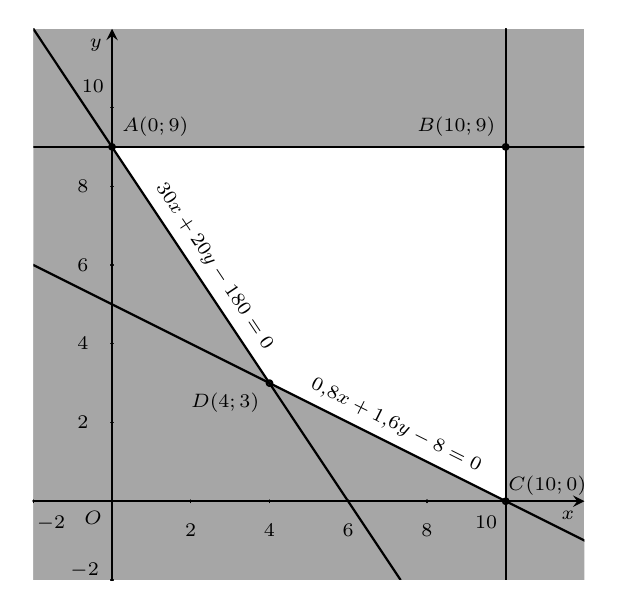
\begin{tikzpicture}[line join=round, line cap=round,>=stealth,thick,scale =.5]
				%	\tikzset{every node/.style={scale=0.9}}
				\begin{scope}
					\clip (-2,-2) rectangle (12,12);
					\fill[black!35] (-3,13.5)--(-3,-10.5)--(13,-10.5)--cycle;
					\fill[black!35] (-15,12.5)--(-15,-2.5)--(15,-2.5)--cycle;
					\fill[black!35] (10,-2)--(12,-2)--(12,12)--(10,12)--cycle;
					\fill[black!35] (-2,9)--(-2,12)--(12,12)--(12,9)--cycle;
					\draw (-2,12)--(7.33,-2)node [pos=0.45, above, sloped,font=\scriptsize] {$30x+20y-180=0$};
					\draw (-14,12)--(14,-2) node [pos=0.75, above, sloped,font=\scriptsize] {$0{,}8x+1{,}6y-8=0$};
					\draw (10,-2)--(10,12);
					\draw (-2,9)--(12,9);
				\end{scope}
				\draw[->] (-2,0)--(12,0) node[below left,font=\scriptsize]{$x$};
				\draw[->] (0,-2)--(0,12) node[below left,font=\scriptsize]{$y$};
				\draw (0,0) node[below left,font=\scriptsize]{$O$};
				\foreach \x/\g in {-2/-50,2/-90,4/-90,6/-90,8/-90,10/225}
				\draw[thin] (\x,1pt)--(\x,-1pt) node [shift={(\g:10pt)},font=\scriptsize] {$\x$};
				\foreach \y/\g in {-2/160,2/180,4/180,6/180,8/180,10/130}
				\draw[thin] (1pt,\y)--(-1pt,\y) node [shift={(\g:10pt)},font=\scriptsize] {$\y$};
				\draw (0,9) circle (2pt) node [above right,font=\scriptsize] {$A(0;9)$};
				\draw (10,9) circle (2pt) node [above left,font=\scriptsize] {$B(10;9)$};
				\draw (10,0) circle (2pt) node [shift={(20:16pt)},font=\scriptsize] {$C(10;0)$};
				\draw (4,3) circle (2pt) node [below left,font=\scriptsize] {$D(4;3)$};
			\end{tikzpicture}	
		\end{center}
		Ta thấy các điểm $A(0;9)$, $B(10;9)$, $C(10;0)$, $D(4;3)$.\\
		Khi này ta có $C_A=36$, $C_B=86$, $C_C=50$, $C_D=32$.\\
		Vậy chi phí thấp nhất là $32$ triệu đồng khi thuê $4$ xe loại $A$ và $3$ xe loại $B$.}
\end{ex}

\begin{ex}%[0H4V3-2]
	\immini[thm]{Bạn An đứng ở sân thượng của tòa nhà và quan sát chiếc diều, nhận thấy góc giữa phương nhìn từ mắt của An tới chiếc diều và phương nằm ngang là $\alpha=50^\circ$. Khoảng cách từ sân thượng tòa nhà tới mắt của An là $1{,}7$ m. Cùng lúc đó, ở dưới chân tòa nhà theo phương thẳng đứng với vị trí của An, bạn Bình cũng quan sát chiếc diều đó và thấy góc giữa phương nhìn từ mắt của Bình tới chiếc diều và phương nằm ngang là $\beta=75^\circ$. Khoảng cách từ mặt đất tới mắt của Bình là $1{,}6$ m. Biết chiều cao của tòa nhà là $h=22$ m (hình vẽ).
		Hỏi chiếc diều ở vị trí cách mặt đất bao nhiêu mét (các phép toán làm tròn kết quả đến hàng phần chục)?}
	{\begin{tikzpicture}[scale=0.8, font=\footnotesize, line join=round, line cap=round, >=stealth,]
			\begin{scope}[shift=({0.2,0})]
				% Con dieu
				\filldraw[fill=orange!50,draw=brown] (3.5,5)--(2.8,4.9)--(2.6,5.5)--(3.2,5.6)--cycle;
				\draw[color=brown] (3.5,5)--(2.6,5.5) (2.8,4.9)--(3.2,5.6);
				\draw[line width=0.5mm,rounded corners,color=orange] (3.5,5)--(3.7,5.1)--(4,4.9)--(4.4,5.1) (3.5,5)--(3.6,4.8)--(3.9,4.9)--(4.5,5);
			\end{scope}
			% Cac chi tiet con lai
			\draw (0,0)--(2,0)--(2,4.2)--(0,4.2)--(0,0);
			\draw (1,0)--(1,4.2);
			\foreach \x in {0.7,1.4,...,3.5}{
				\draw (0,\x)--(2,\x);
			}
			\path
			(2,4.55) coordinate (A)
			(3.2,4.55) coordinate (A')
			(2,0.35) coordinate (B)
			(3.2,0.35) coordinate (B')
			(3.2,5.25) coordinate (C)
			;
			\draw (3.2,0)--(2,0)--(A)--(C)--(B);
			\draw[dashed] (C)--(3.2,0) (A)--(A') (B)--(B');
			\foreach \d/\g in {} \fill (\d)node[shift={(\g:0.3)}]{$\d$} circle(1pt);
			\pic[draw,angle radius=4mm,angle eccentricity=1.5] {angle = A'--A--C};
			\pic[draw,angle radius=4mm,angle eccentricity=1.5] {angle = B'--B--C};
			\pic[draw,angle radius=5mm,angle eccentricity=1.5] {angle = B'--B--C};
			\fill (0,1.4)node[shift={(180:0.3)}]{$h$};
			\fill (A)node[shift={(13:0.65)}]{$\alpha$};
			\fill (B)node[shift={(40:0.75)}]{$\beta$};
	\end{tikzpicture}}
	% \par
	% \shortans[]{34{,}1}
	\loigiai{
		\begin{center}
			\begin{tikzpicture}[scale=0.8, font=\footnotesize, line join=round, line cap=round, >=stealth,]
				% Cac chi tiet con lai
				\draw (0,0)--(2,0)--(2,4.2)--(0,4.2)--(0,0);
				\draw (1,0)--(1,4.2);
				\foreach \x in {0.7,1.4,...,3.5}{
					\draw (0,\x)--(2,\x);
				}
				\path
				(2,4.55) coordinate (N)
				(3.2,4.55) coordinate (A')
				(2,0.35) coordinate (M)
				(3.2,0.35) coordinate (B')
				(3.2,5.25) coordinate (D)
				;
				\draw (3.2,0)--(2,0)--(N)--(D)--(M);
				\draw[dashed] (D)--(3.2,0) (N)--(A') (M)--(B');
				\foreach \d/\g in {N/180,M/180} \fill (\d)node[shift={(\g:0.3)}]{$\d$} circle(1pt);
				\pic[draw,angle radius=4mm,angle eccentricity=1.5] {angle = A'--A--C};
				\pic[draw,angle radius=4mm,angle eccentricity=1.5] {angle = B'--B--C};
				\pic[draw,angle radius=5mm,angle eccentricity=1.5] {angle = B'--B--C};
				\fill (0,1.4) node[shift={(180:0.3)}]{$h$};
				\fill (A) circle (1.5pt) node[shift={(13:0.65)}]{$\alpha$};
				\fill (B) circle (1.5pt) node[shift={(40:0.75)}]{$\beta$};
				\fill (C) circle (1.5pt) node[shift={(90:0.2)}]{$D$};
				\fill (B') circle (1.5pt) node[shift={(0:0.3)}]{$H$};
				\fill (3.2,4.55) circle (1.5pt) node[shift={(-45:0.3)}]{$K$};
				\fill (3.2,0) circle (1.5pt) node[shift={(-90:0.3)}]{$E$};
			\end{tikzpicture}
		\end{center}
		Đặt tên các điểm như hình vẽ với $M$, $N$ lần lượt là vị trí mắt của Bình, An. Ta có $MN=22{,}1$\,(m).\\ 
		Xét tam giác $MND$ có\\ $\widehat{MND}=90^\circ+50^\circ=140^\circ$, $\widehat{NMD}=90^\circ-75^\circ=15^\circ$, $\widehat{MDN}=180^\circ-140^\circ-15^\circ=25^\circ$.\\
		Áp dụng định lí sin cho tam giác $MND$ ta có $\dfrac{MD}{\sin N}=\dfrac{ND}{\sin M}=\dfrac{MN}{\sin D}$.\\ 
		Suy ra $MD=\dfrac{MN\cdot\sin N}{\sin D}=\dfrac{22{,}1\cdot \sin 140^{^\circ}}{\sin 25^{^\circ}} \approx 33{,}6$\,(m).\\ Xét tam giác $MHD$ vuông tại $H$, ta có
		$HD=MD\cdot \sin 75^\circ\approx 33{,}6\cdot \sin 75^\circ=32{,}5$\,(m).\\
		Do đó $DE\approx 1{,}6+32{,}5=34{,}1$\,(m).\\
		Vậy chiếc diều ở vị trí cách mặt đất khoảng $34{,}1$\,(m).
	}
\end{ex}